\documentclass[12pt]{article}
\usepackage[utf8]{inputenc}
\usepackage{graphicx} % For including images
\usepackage{geometry} % For page size and margins
\geometry{a4paper, margin=0.8in}

\title{Hospital Management System: Architectural Documentation}
\author{Muhammad Rehan \\ 22P-9106}
\date{Assignment 02}
\begin{document}

\maketitle

\section*{Assignment Abstract}
This assignment presents a comprehensive architectural overview of the Hospital Management System (HMS), outlined through four distinct views: Logical, Development, Process, and Physical. Each view addresses specific aspects of the system's functionality, scalability, and performance. The Logical View details the system's core functionalities and user interactions. The Development View breaks down the system into modular components, highlighting the software development structure. The Process View describes the dynamic interactions and workflows essential for system operation. The Physical View maps the deployment of the system onto hardware and network infrastructure. This architectural assignment aims to ensure that the HMS is robust, secure, and capable of adapting to the evolving needs of modern healthcare environments.

\section*{Logical View}
\subsection*{Overview}
The Logical View clarifies the system’s key components and their interactions, focusing on meeting the functional requirements derived from user stories. This view includes core entities such as Patients, Doctors, Nurses, Receptionists, Lab Assistants, Pharmacists, and Billing staff, outlining their responsibilities and interconnections.

\subsection*{Purpose}
This view aids in visualizing the system’s architecture from a functionality standpoint. It shows how different user roles interact with the system to perform their tasks, which supports effective management of the system’s complexity.

\subsection*{Diagram}
\begin{figure}[h!]
\centering
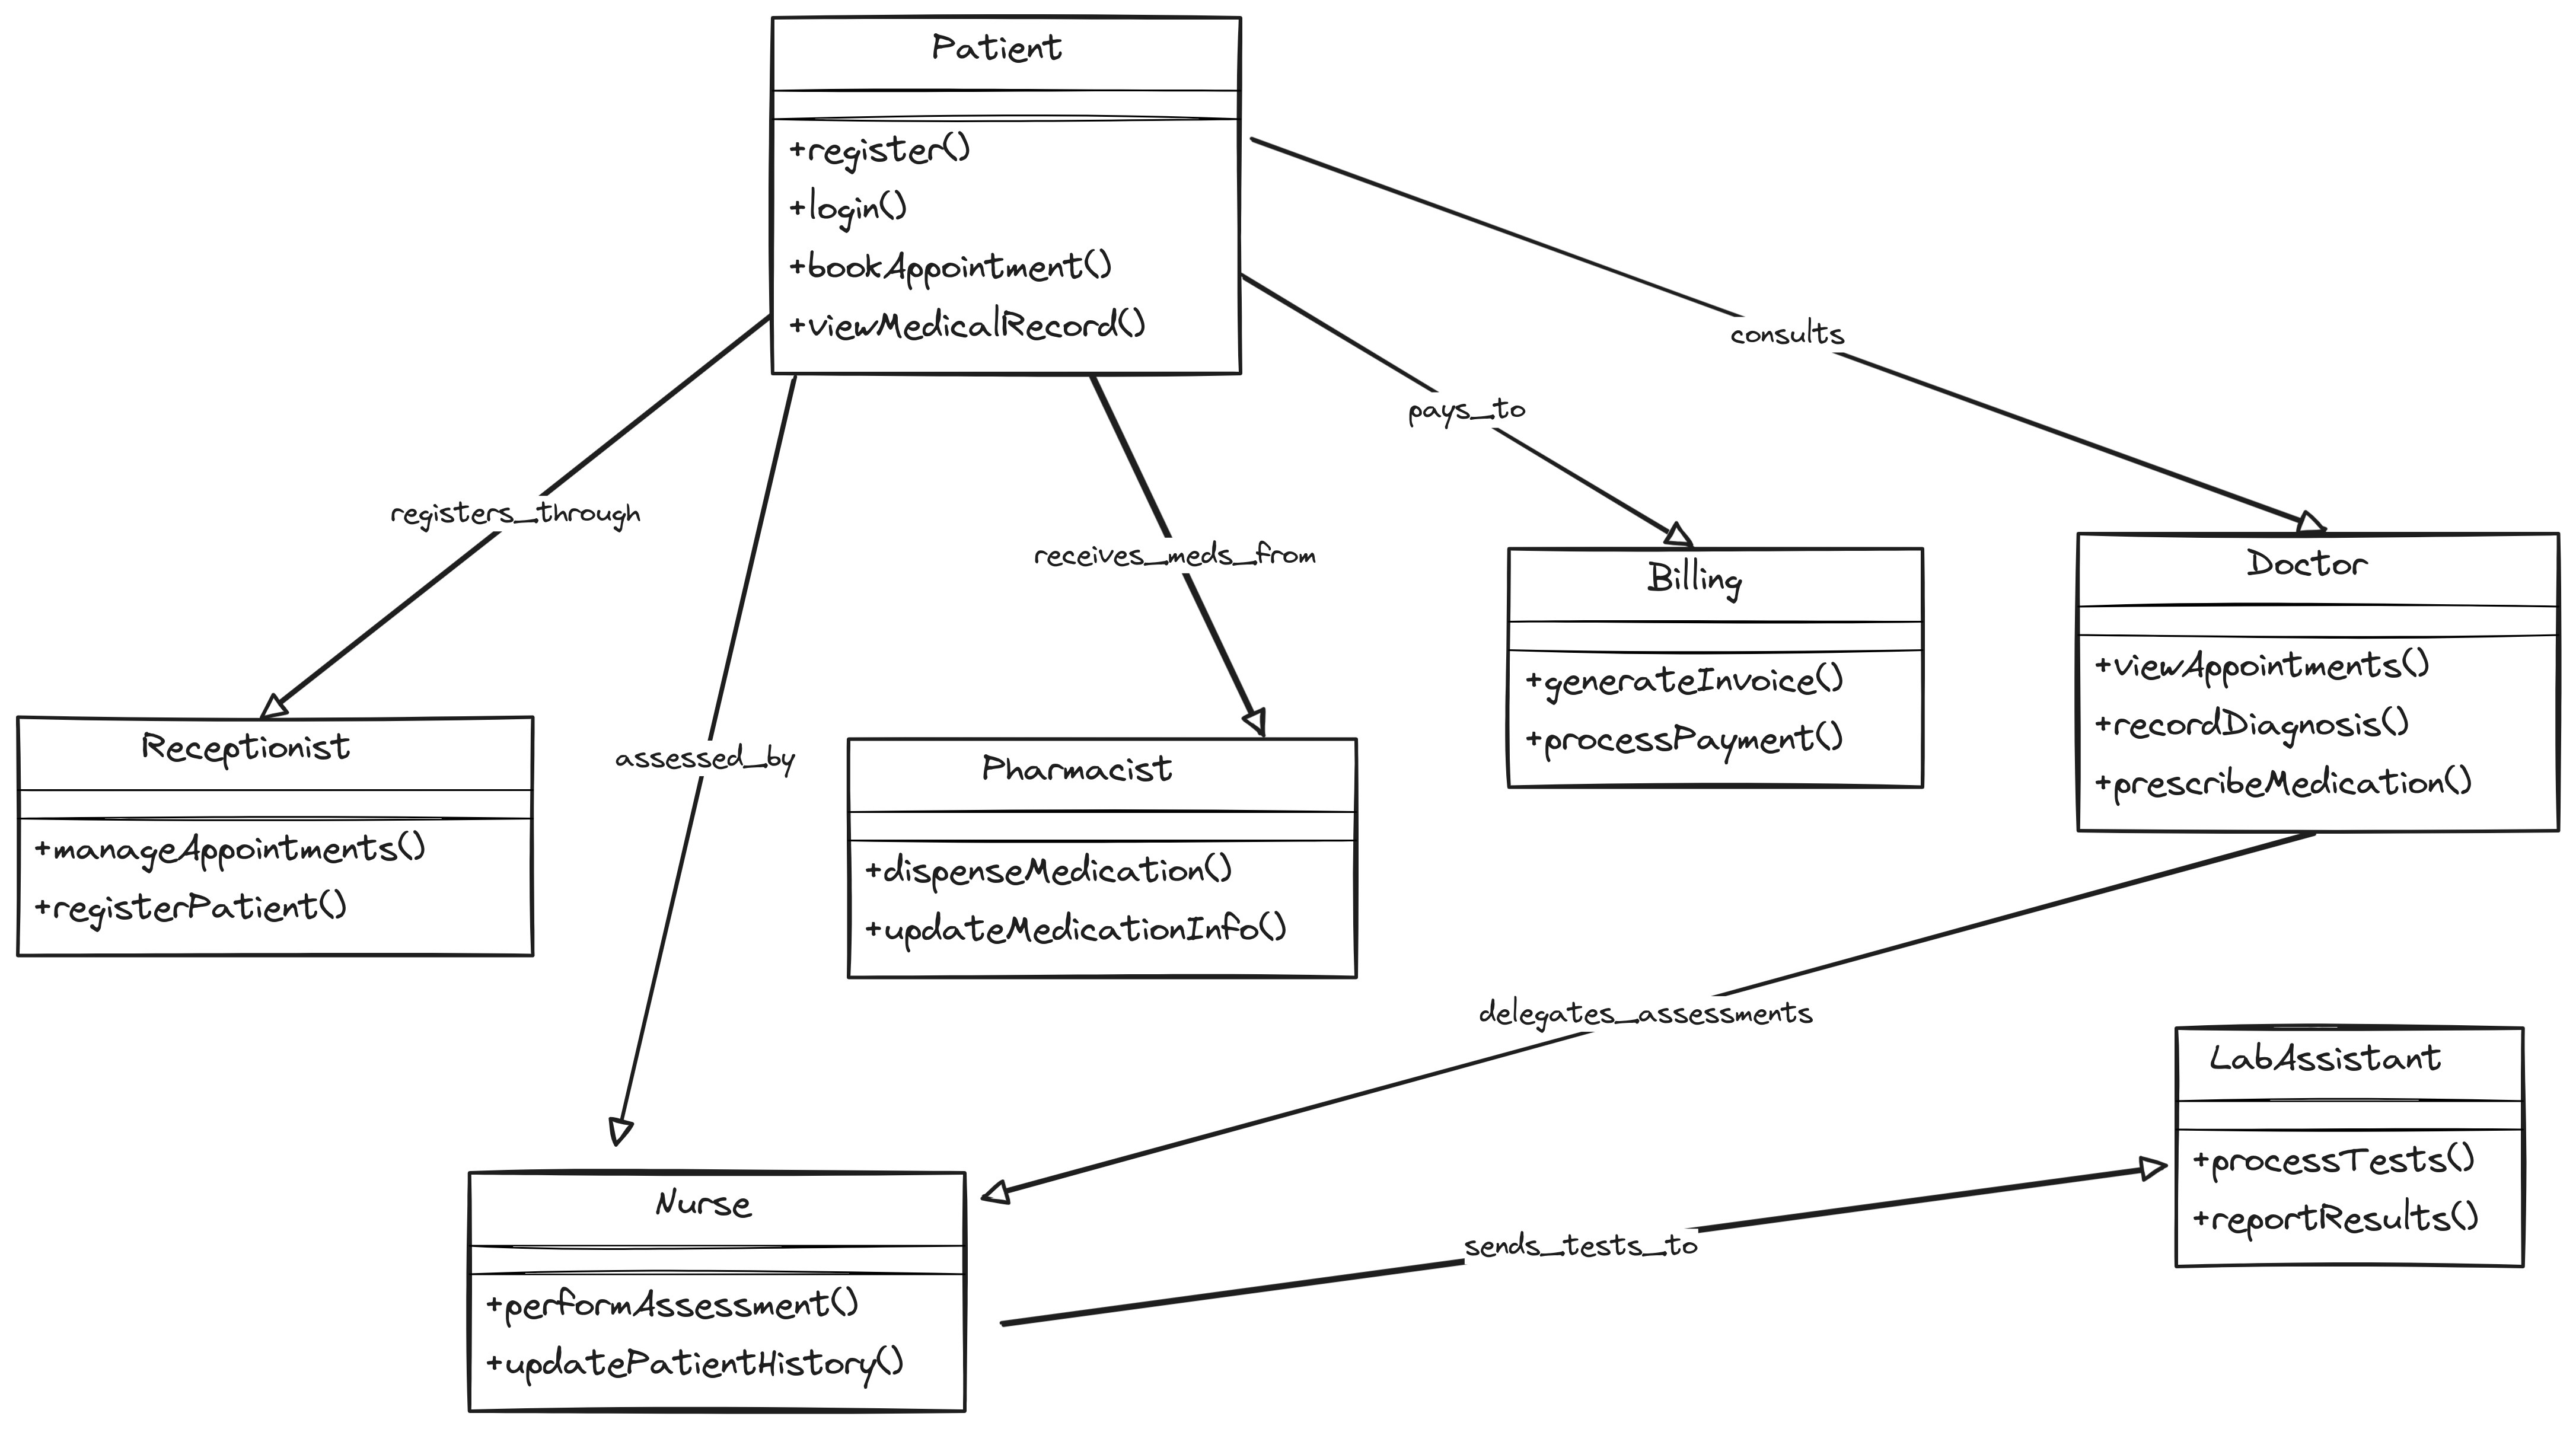
\includegraphics[width=0.8\textwidth]{Logicalview.png}
\caption{Logical View Diagram}
\end{figure}


\newpage


\section*{Development View}
\subsection*{Overview}
The activity diagram in the Development View provides a dynamic representation of the system’s operational workflows, focusing on the sequence of actions involved in a typical user interaction with the Hospital Management System. This diagram traces the steps a patient follows, from logging into the system to completing payment for services received, illustrating the interaction between different system components such as the patient interface, healthcare providers, and administrative modules.

\subsection*{Purpose}
The primary purpose of the activity diagram is to visually communicate the flow of activities that occur within the system from start to finish. It serves as a vital tool for understanding and documenting the process logic and operation flow, especially useful for developers, ensuring that the system’s functionality aligns with user needs and expectations.

\subsection*{Diagram}
\begin{figure}[h!]
\centering
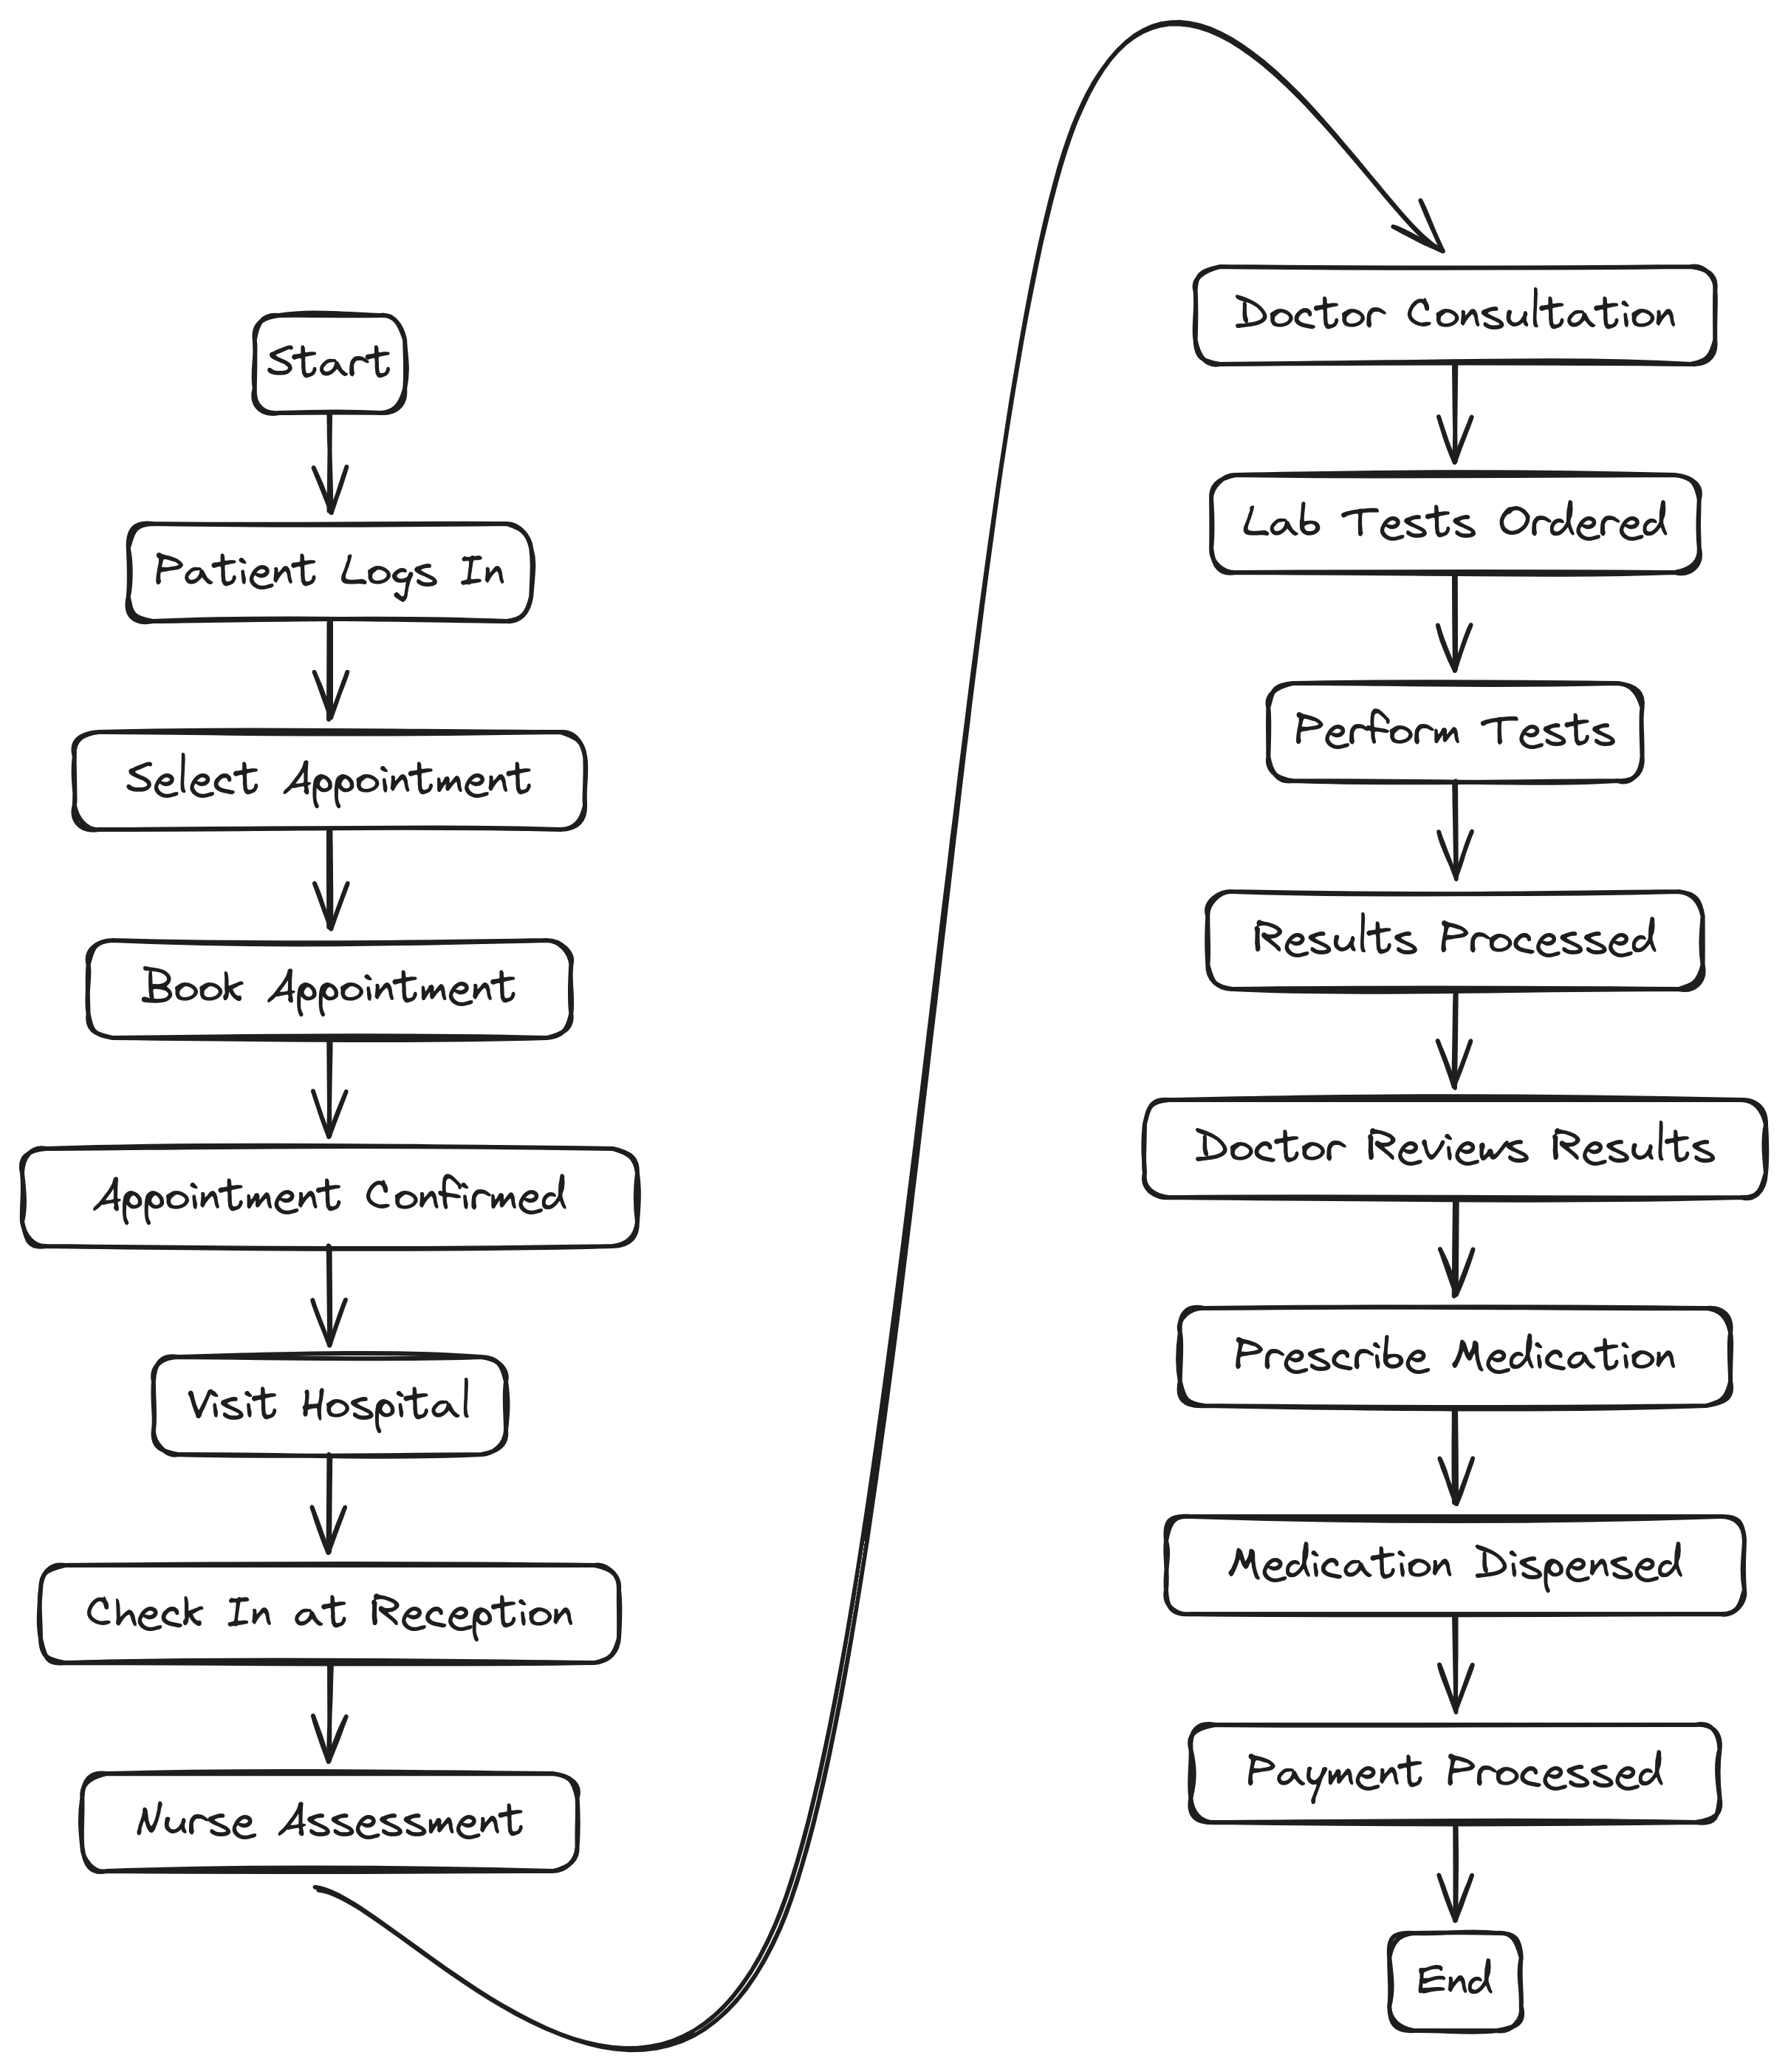
\includegraphics[width=0.8\textwidth]{activity.png}
\caption{Development View Diagram}
\end{figure}



\newpage


\section*{Process View}
\subsection*{Overview}
The Process View focuses on the dynamic aspects of the system, particularly how processes operate and interact over time. This view is crucial for understanding the system's behavior during its execution, especially in terms of process coordination, concurrency, and distribution.

\subsection*{Purpose}
The purpose of the Process View is to detail the runtime behavior of the system, showing how various processes are made to handle tasks efficiently. This view is essential for identifying performance drawbacks, ensuring proper load balancing, and optimizing response times.

\newpage


\subsection*{Diagram}
\begin{figure}[h!]
\centering
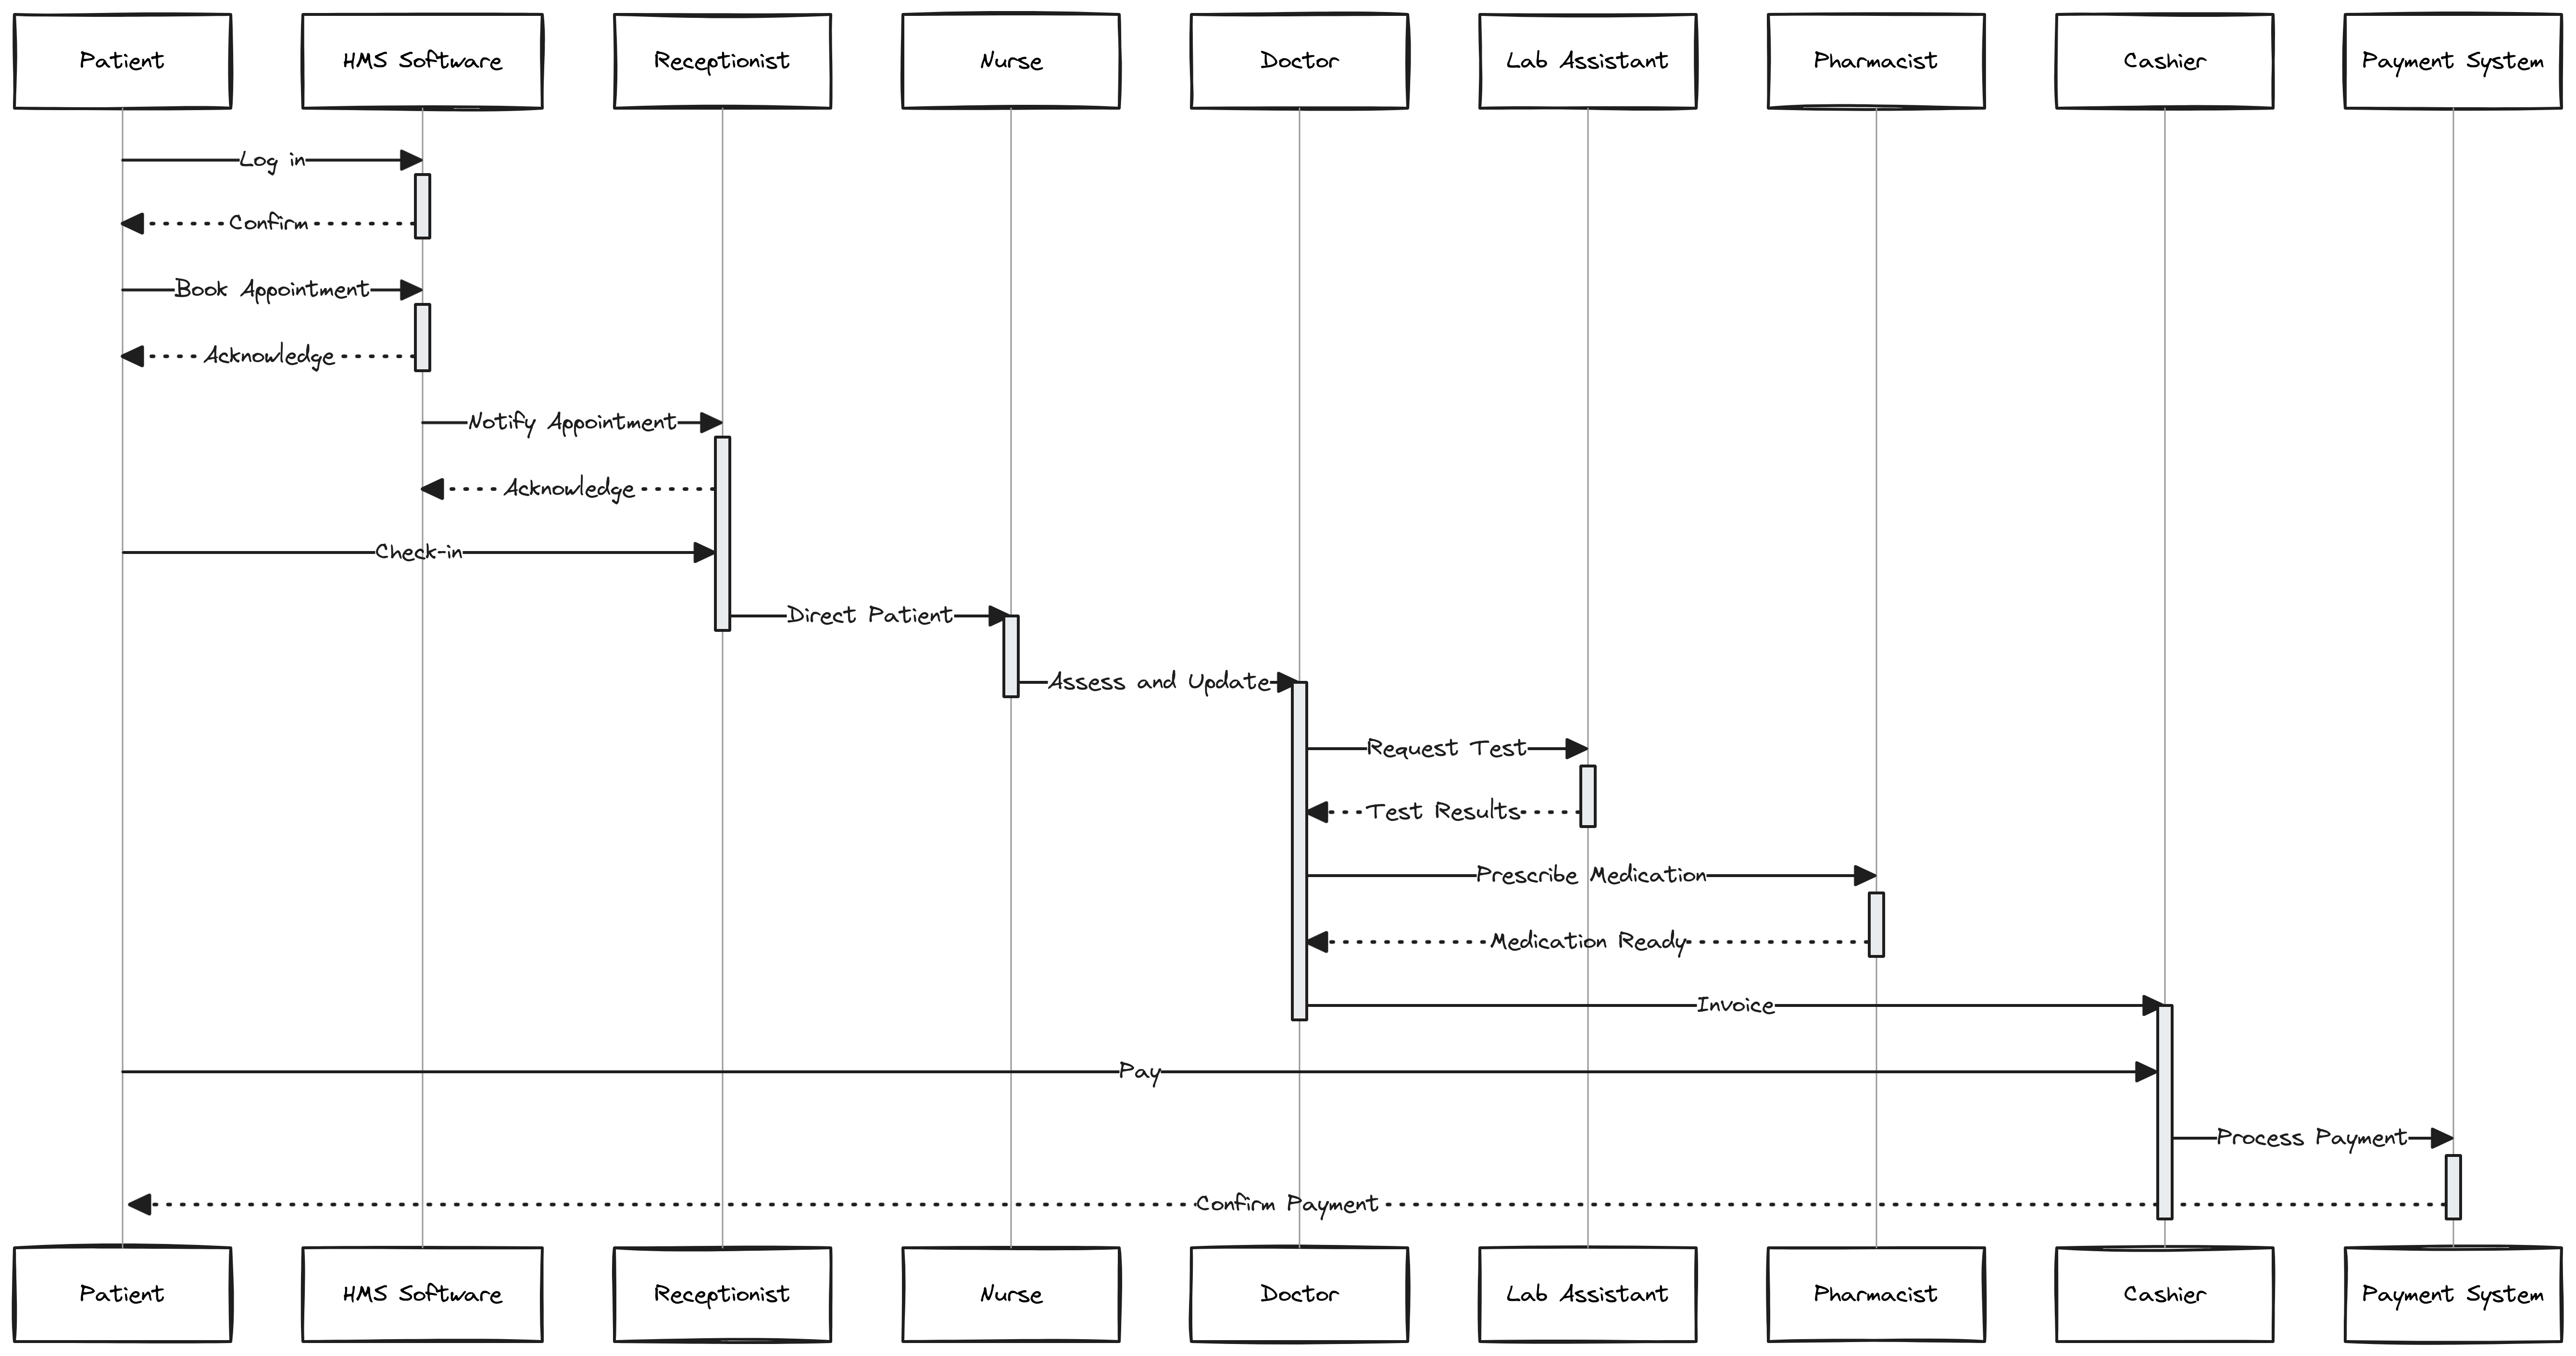
\includegraphics[width=0.8\textwidth]{process.png}
\caption{Process View Diagram}
\end{figure}




\section*{Physical View}
\subsection*{Overview}
The Physical View describes how the software components are deployed on the hardware infrastructure, including details about servers, network, and client devices. This view is essential for ensuring that the system's performance, scalability, and reliability meet the operational requirements of the hospital.

\subsection*{Purpose}
The purpose of the Physical View is to showcase the system's deployment strategy, which helps in understanding how components communicate over the network and how data flows between different parts of the system. It also focuses on redundancy, failover mechanisms, and load balancing to enhance system availability and performance.





\subsection*{Diagram}
\begin{figure}[h!]
\centering
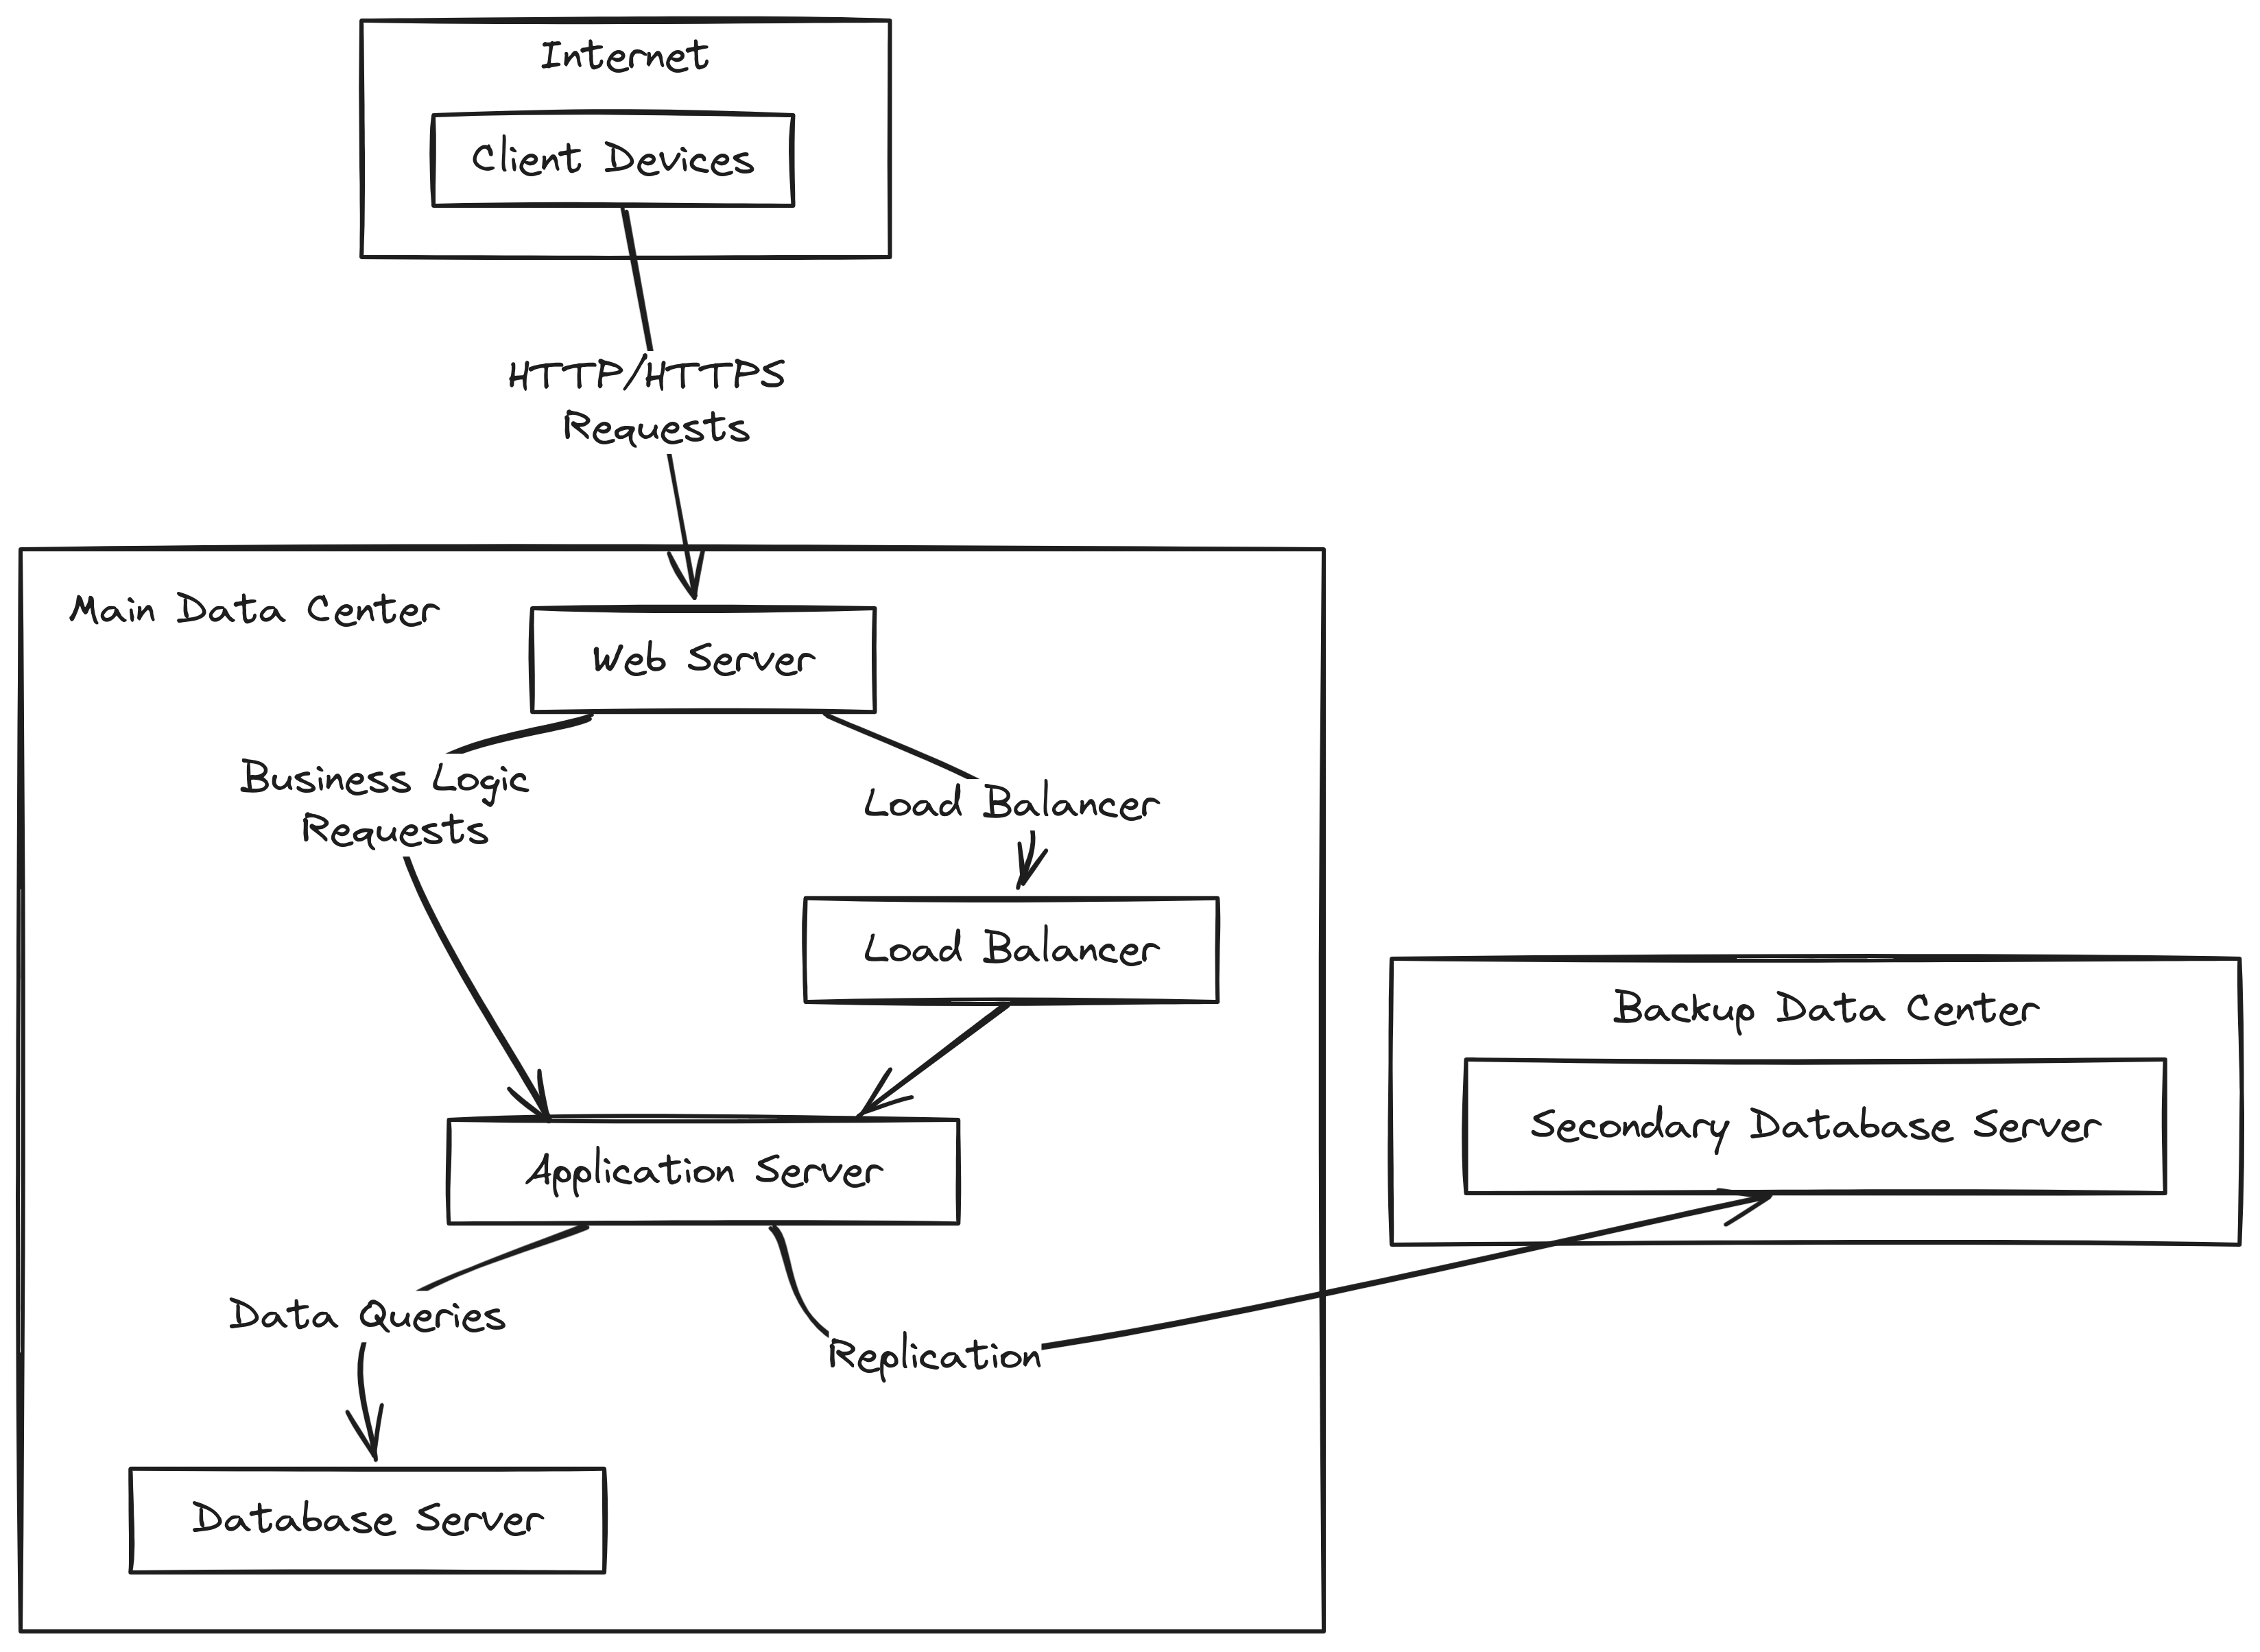
\includegraphics[width=0.8\textwidth]{physical.png}
\caption{Physical View Diagram}
\end{figure}



\newpage


\section*{Key Considerations}
The diagrams covers the breadth and depth of the architectural views for the given case study in the assignment, containing the abstracting essential details. But, making highly complex diagrams at this point is not practical.

\noindent\hrulefill


\end{document}
